\documentclass[a4paper, 12pt]{article}

\usepackage[brazilian]{babel}
\usepackage[utf8]{inputenc}
\usepackage[T1]{fontenc}
\usepackage[a4paper]{geometry}
\usepackage{amsmath}
\usepackage{amssymb}
\usepackage{indentfirst}
\usepackage{hyperref}
\usepackage{graphicx}
\renewcommand{\rmdefault}{ptm}
\graphicspath{{./images/}}

\title{Relatório EP1 de MAC0209}
\author{Beatriz Marouelli, Bruno Scholl, João Henrique, 
\\ Leonardo Lana, Lucas Yau, Victor Seiji}
\date{10 de abril de 2017}

\begin{document}
\maketitle

\section*{Introdução}
Neste primeiro experimento foi proposto simularmos o movimento retilíneo
uniforme (MRU), na qual o corpo se movimento em uma trajetória retilínea com
velocidade constante, e o movimenta retilíneo uniformemente variado (MRUV),
o movimento, novamente, será retilíneo porém desta vez, a velocidade varia
segundo uma aceleração constante.

\section*{Método}
Utilizamos o acelerômetro do celular através do Physics Tool Box para
determinarmos a aceleração. Para facilitar, toda pessoa que fizesse o experimento 
tanto em MRU quanto MRUV, ficava parada com o celular estável na mão por 5 segundos, 
assim ao analizarmos os dados teríamos um parâmetro para a estabilidade, o mesmo 
foi feito ao fim do experimento.

A fim de atingirmos uma precisão maior, pedimos auxílio de outro grupo, desta
forma poderíamos ter 6 cronômetros, dois alinhados em lados opostos do trajeto
a cada 10 metros e posteriormente, um a cada 5 alternando os lados.

Usamos o mesmo celular para todos os experimentos para evitar inconsistências,
que poderiam surgir caso os acelerômetros (sensor) dos celulares fossem diferentes.

Para a planilha de dados amostrais, usamos média aritmética simples.

Para modelar os dados obtidos pelo Physics Tool Box usamos as equações: \\
\\
Para o Movimento Retilíneo Uniforme:
$$v = \frac{\Delta x}{\Delta t} \quad a = \frac{\Delta v}{\Delta t}$$
Para o Movimento Retilíneo Unfiormente Variado:
$$x = x_0 + v_0 t + \frac{a}{2} t^2 \quad v = v_0 t + at$$

\section*{Verificação de Programa}
O programa usa do método de euler para o cálculo. Ele calcula os Delta Ts
($\delta t$) entre cada par de posições dos cronômetros. Com isso, ele assume
que as separações entre cronômetros são de 10m, e calcula as velocidades de
acordo com os Deltas de posição ($\delta S$) assim, a velocidade na posição dada
é calculada por $\frac{\delta S}{\delta t}$.
A mesma coisa para o cálculo das acelerações. A aceleração na posição dada é
calculada por $\frac{\delta v}{\delta t}$.

\section*{Análise}
Ao calcularmos manualmente usando os dados amostrais e usando os dados das
tabelas \textit{.csv} obtivemos erros em torno de 30\% para as velocidades.
E erros muito grandes, acima de 50\%, para a aceleração. 

\section*{Interpretação}
No MRU, conseguimos manter uma velocidade constante em boa parte dos experimentos.
Porém ao analisar o MRUV, vimos que a aceleração sofre algumas alterações
consideráveis durante os experimentos.

As dúvidas que surgiram durante o experimento foram: possíveis instrumentos para
regular aceleração e velocidade; métodos para diminuir a margem de erro do
sensor; como fazer os experimentos com o minímo de precisão só com 5 pessoas.

\section*{Critícas}
Para os modelos fisícos não houve grandes avanços, usamos somente modelos
simples os quais já dominávamos. A grande novidade foi a dificuldade em coletar
dados minimizando variavéis que poderiam acentuar os erros, nos quais o fator
humano (manter a velocidade/aceleração constante, atraso para parar o
cronômetro, estabilizar o celular na mão) já cria uma margem de erro considerável. 

No escopo computacional, já tinhamos conhecimento de \textit{\textbf{python}} e
\textit{\textbf{matplotlib}}. A parte a qual nos tomou mais tempo foi consertar
os dados das tabelas \textit{.csv}, para que elas pudessem ser utilizadas em
nossos programas.

\section*{Link do Vídeo}
O link para o vídeo do experimento é:
\url{https://www.youtube.com/watch?v=z1ODFN4LaS8}

\section*{Dados}
    \begin{figure}
    \centering
    Dados amostrais Beatriz Marouelli
    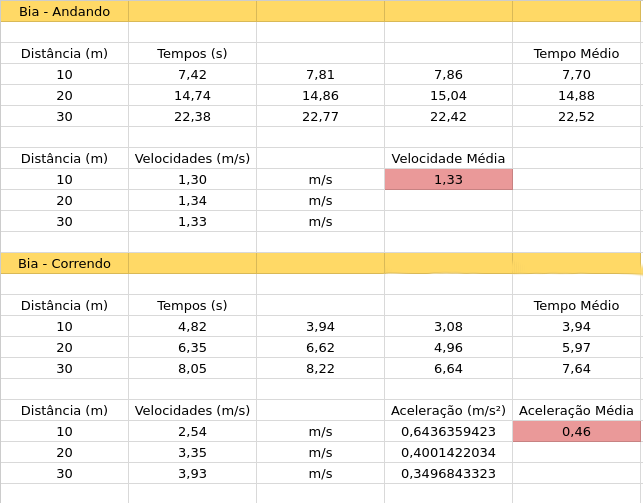
\includegraphics[scale=0.45]{Bia.png}
    \\ Dados amostrais Bruno Scholl
    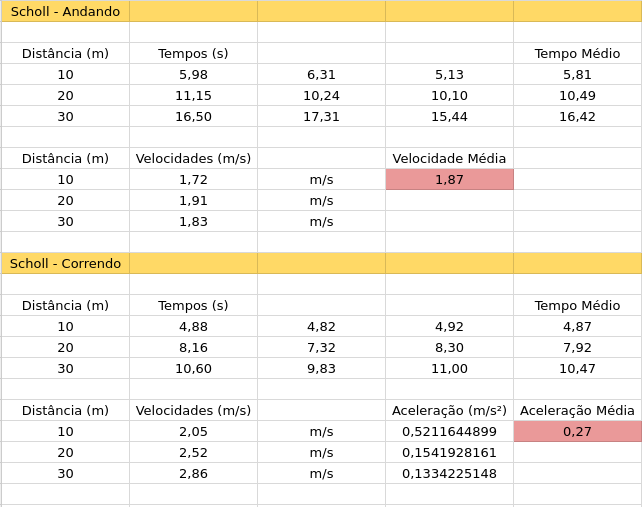
\includegraphics[scale=0.45]{Scholl.png}
    \\ Dados amostrais Victor Seiji 
    \end{figure}
\section*{Contribuições}
\textbf{Beatriz Marouelli}: cobaia, plotou os gráficos do csv, 
fez o mru.py, organização do grupo em geral e edição do vídeo.

\textbf{Bruno Scholl}: cobaia, planilha dos dados amostrais.

\textbf{João Henrique}: plotou os dados amostrais.

\textbf{Leonardo Lana}: relatório, organização dos arquivos e dados.

\textbf{Lucas Yau}: script de correção dos csv's.

\textbf{Victor Seiji}: cobaia, corrigiu erros no MRU.py (Agora Simulation.py) e ajudou na planilha.

\textbf{Todos}: ajudaram no experimento.
\end{document}
